\documentclass[../main.tex]{subfiles}
\begin{document}
\subsection{Active Learning}
Active Learning (AL) presents a promising approach to address one of the most resource-intensive stages of the SR: title and abstract screening. In the context of SRs, where the volume of potentially relevant literature is vast and growing, AL offers a method to significantly reduce the manual workload while maintaining high accuracy in document selection.
Traditional systematic review methods require domain experts to manually screen all titles and abstracts identified in the initial search phase. This process is time-consuming and costly, especially given the increasing volume of published research. AL aims to optimise this process by intelligently selecting which documents should be reviewed by human experts, potentially saving significant time and resources.
By applying AL techniques to the screening process, we can:
\begin{itemize}
    \item Prioritise potentially relevant documents for expert review
    \item Reduce the overall number of documents that require manual screening
    \item Potentially identify relevant documents that might be missed in manual screening due to human fatigue or error
    \item Accelerate the overall SR process without compromising on quality
\end{itemize}

Deep-learning models have traditionally relied on large-labelled datasets for training. However, this approach contrasts sharply with real-world scenarios, particularly in specialised domains such as medicine. Although data collection is relatively straightforward in these fields, labelling is often time-consuming and requires expert knowledge \cite{smith_less_2018, hoi_batch_2006}. This disparity presents a significant challenge to optimise model performance with a limited number of labelled examples. This challenge is particularly relevant to the screening process in SRs, where we currently ask experts to screen all titles and abstracts returned from the identification phase. However, we would want to move to a scenario where minimal expert screening is sought from research returned from the identification phase, whose screening can then be safely extrapolated to a larger pool.

Active learning (AL) studies how to do just this. Through AL terms, it attempts to use a sampling policy $\pi$ to select samples $\mathbf{T}{C,i}$ from an unlabelled dataset $\mathbf{T}{U,i}$ and pass them to an oracle for labelling and added to a known dataset $\mathbf{T}_{K,i}$. Technology-Assisted Review (TAR), also known as Computer-Assisted Review or Predictive Coding, is a process that uses machine learning to assist in document review tasks. In the context of SRs, the TAR applies AL principles to streamline the selection process of titles and abstracts to screen. By iteratively training a machine learning model on human-labelled examples, TAR can prioritise potentially relevant documents for expert review, significantly reducing manual workload and, in some cases, exceeding human ability \cite{grossman_technology-assisted_2010}. This approach aligns closely with the goals of AL in SRs, as it aims to maximise the efficiency of expert input while maintaining high accuracy in document classification. 

Different approaches can be taken to AL, such as membership query synthesis \cite{angluin_queries_1988}, stream-based selective \cite{akinseloyin_novel_2024} and pool-based sampling \cite{lewis_sequential_1994}. These approaches are divided on how much of the unlabelled dataset ($\mathbf{T}{U, i}$) that a model has access to when utilising a policy $\pi$ for the selection of data points to be labelled $\mathbf{T}{C,i}$. In pool-based sampling, the entire unlabelled dataset, $\mathbf{T}{U,i}$, is evaluated in the selection of $\mathbf{T}{C,i}$, in stream-based selective sampling, datapoints are evaluated one at a time, and in membership query synthesis, synthetic data are generated from an underlying natural distribution. As we are concerned solely with the subprocess of title and abstract screening, it aligns strongly with pool-based sampling as the entire unlabelled dataset is known ahead of time and will be the approach used within this PhD. Figure \ref{fig:pool_based_query} outlines the AL cycle with pool-based querying.

\begin{figure}
\centering
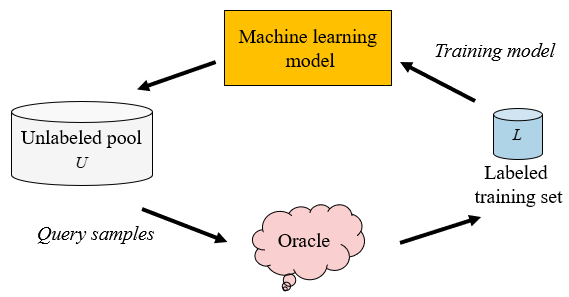
\includegraphics[width=0.5\linewidth]{sections//images/pool_based_strategy.png}
\caption{Overview of a pool-based query strategy for AL, replicated\cite{ren_survey_2021}}.
\label{fig:pool_based_query}
\end{figure}

The oracle ($O$) within this PhD will denote a human-verified label resulting from screening potential research for inclusion within the SR within the title and abstract screening stage. Domain experts typically perform this. More concretely, $O$ can be considered a function $O(x) = y$ where $X$ is a representation, such as embedding the research title and abstract, and $y$ is the assigned category (included or excluded). We assumed that for each datapoint ($x$), $O$ provides a single judgement ($y$), which is always correct and do not concern ourselves with any potential intercoder agreement or bias within that decision process \cite{artstein_survey_2008}.

The broader literature has evaluated the effects of the choice of $\pi$. Traditionally, $\pi$ used the sigmoid response of the final layer of a model as a proxy of confidence, which is not a reliable measure, as these responses tend to be overly confident \cite{pearce_understanding_2021}. The use of the softmax response has been shown, in some cases, to be worse than random sampling \cite{wang_new_2014}. However, the effect of the choice of $\pi$ in combination with the final output layer in this specific domain (i.e. the SR process) is unknown, and this remains an active area of research which will not be covered during the PhD. The author uses techniques such as temperature scaling to effectively combat overly confident soft-max responses \cite{guo_calibration_2017}.


\begin{table*}[t]
    \centering
    \footnotesize

    \begin{tabular}{|c|c|>{\raggedright\arraybackslash}p{11cm}|}
        \hline
        \textbf{Notation}    & \textbf{Explanation}                            & \textbf{Notes}                                                                                \\
        \hline
        \(\textbf{T}\)       & Total dataset                                   & e.g. Research gathered after Identification phase of the selection process.                   \\
        \hline
        \(i\)                & Iteration                                       & A single cycle within the active learning process.                                            \\
        \hline
        \(\textbf{T}_{K,i}\) & Known datapoints per iteration                  & e.g. research that has been screened by a reviewer                                            \\
        \hline
        \(\textbf{T}_{U,i}\) & Unknown datapoints per iteration                & e.g. research that has not been screened by a reviewer                                        \\
        \hline
        \(\textbf{T}_{C,i}\) & A subset of \(\textbf{T}_{U,i}\) to be labelled & chosen by a policy, datapoints to be screened by a reviewer.                                  \\
        \hline
        $\pi$                & Policy                                          & How \(\textbf{T}_{U,i}\) is selected, e.g. uncertainty, random, certainty, diversity sampling \\
        \hline
        O                    & Oracle                                          & Often a domain expert, who assigns labels to unscreened research.                             \\
        \hline
        \(T_R\)              & Total Relevant Documents                        & All research that should be included in a systematic review.                                  \\
        \hline
        \(T_{IR}\)           & Total Irrelevant Documents                      & All research that should not be included in a systematic review.                              \\
        \hline
    \end{tabular}
    \caption{Notation used for active learning within this review}
    \label{tab:notation}
\end{table*}


In the author's mind, it is unclear the exact difference between continuous/online active learning (CAL) and AL, and indeed, it seems that much of the current literature refers to CAL when, in fact, it means AL. Some authors refer to eliminating models between iterations and the process occurring in discrete rounds as AL \cite{settles_active_2009}. Cormack differentiates the two based on objectives, with the aim of CAL being to find and review as many of the responsive documents as possible, as quickly as possible, and AL is to produce the best classier possible, considering the level of training effort (which are subtlely different objectives) \cite{cormack_autonomy_2015}. For this research, we will use continuous to denote the incremental streaming of newly available information to any model. 
\end{document}